\begin{figure}[!h]
  \centering
  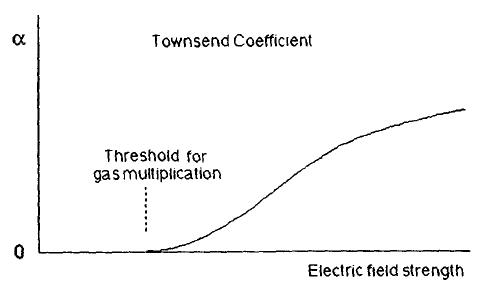
\includegraphics[width=.5\linewidth]{townsend_coefficient}
  \caption{The first Townsend coefficient as a function of the applied field\autocite{Knoll:RadMeasurement}.}
  \label{fig:town_coeff}
\end{figure}
When a ionizing particle interacts with neutral molecules, an \emph{ion pair} is
formed. This can happen either by direct interaction with the incident radiation
or by interaction with secondary electrons that gained enough kinetic energy to
ionize the molecules.

While for a low value of the field electron-ion pair simply drift towards the
electrodes, above a certain threshold of the filed, electrons rapidly gain
kinetic energy and if it is greater than the ionization energy of the neutral
gas molecules an additional ion pair is created. The electrons liberated in such
a way, will also gain kinetic energy and, colliding with the neutral gas
molecules, produce additional ionization. This \emph{gas multiplication} process
in which each electron may ionize a neutral gas molecule is known as
\emph{Townsend avalache}, the Townsend equation
\begin{equation}
  \label{eq:townsend}
  \frac{\ud n}{n} = \alpha\, \ud x
\end{equation}
where $\alpha$ is the \emph{first Townsend coefficient}, describes the increase
of the number of electrons ($n$) per unit length ($\ud
x$). Figure~\ref{fig:town_coeff} shows the slope of the $\alpha$ coefficient,
its value is zero when the electron energy is less than the multiplication
threshold and grows with the field strength afterwards. For a cylindrical
symmetry the avalanche increases in the direction of the field, moreover, the
solution of the Townsend equation
\begin{equation}
  \label{eq:townsend_sol}
  n(x) = n(0) e^{\alpha x}
\end{equation}
tells us that the number of electrons has an exponential growth with distance,
thus the growth with distance of the avalanche is even higher.

This multiplication of the charge can give a better signal over noise ration while
diminishing the requirement for an external amplifier. The key point is that the
number of secondary ionization can be kept proportional to the number of primary
ionization but the number of ions can be multiplied by a large factor. As a last
remark, sine the high energy electron avalanche interacts with many atoms, a
variety of different atomic states is formed, thus proportional counters are
sensitive to the gas composition used.

\begin{figure}[!h]
  \centering
  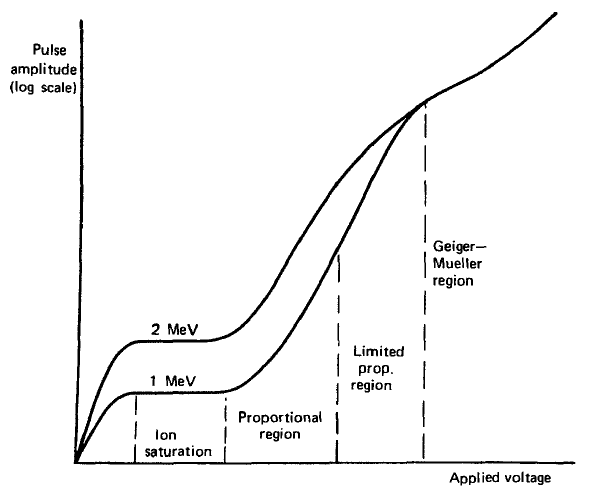
\includegraphics[width=.5\linewidth]{regions_of_operation}
  \caption{Pulse amplitude as a function of the applied voltage\autocite{Knoll:RadMeasurement}.}
  \label{fig:reg_of_operation}
\end{figure}
The amplitude of the observed pulse as a function of the applied voltage is
reported in Figure~\ref{fig:reg_of_operation}, for low values of the voltage,
the field cannot prevent recombination thus the observed the collected charge is
less what was produced by the incident radiation. If the voltage is increased to
the point that the recombination rate becomes negligible, all the charges get
collected by the respective electrode and increasing the voltage further will
not increase the current, this regime is called \emph{ion saturation}. If the
voltage is increased past the ion saturation region, gas multiplication
processes described above will start to occur. This is the region of \emph{true
  proportionality} and is the normal operation condition of proportional
counters. In this region the gas multiplication is linear and the number of
collected charge proportional to the number of ion pairs created by the incident
radiation. Increasing the voltage further will introduce non linear effects
which are beyond the scope of this report (see\autocite{Knoll:RadMeasurement}).

In cylindrical geometry the electric field at radius $r$ is given by:
\begin{equation}
  \label{eq:cyl_el_field}
  E(r) = \frac{V}{r \ln (b / a)}
\end{equation}
where $V$ is the voltage applied between anode and cathode, $a$ is the radius of
the anode wire and $b$ is the active volume radius. Gas multiplication require a
high electric field thus a small anode wire, where $r$ is small, is preferable,
Figure~\ref{fig:wire_el_field} gives a schematic representation of this.
Moreover, in order to achieve a uniform multiplication for the ion pairs created
by the incident radiation, gas multiplication must be confined to a very small
volume around the anode wire so that all the ion pairs are created in the active
volume outside the high field region and the electrons can drift towards the
anode where they can achieve the same multiplication regardless of the original
formation position.
\begin{figure}[!h]
  \centering
  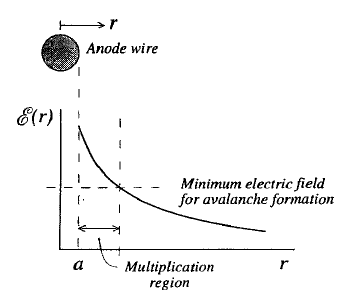
\includegraphics[width=.5\linewidth]{wire_el_field}
  \caption{Electric field dependence on the distance from the anode wire. The
    gas multiplication region is confined to a small volume\autocite{Knoll:RadMeasurement}.}
  \label{fig:wire_el_field}
\end{figure}
%%% Local Variables:
%%% mode: latex
%%% TeX-master: "prop_counter"
%%% End:
